% Training processes every position at once; generation adds one token at a time.
% ---------------------------------------------------------------------------
% style.tex --- shared preamble for every figure in book/figures/tikz/
%
% One style for all figures: Latin Modern, thin black lines, a light grey
% fill, and one accent colour used only to mark what is untrusted or wrong.
% Build with scripts/build_figures.sh; see book/figures/README.md.
% ---------------------------------------------------------------------------
\documentclass[tikz,border=6pt]{standalone}
\usepackage[T1]{fontenc}
\usepackage{lmodern}
\usetikzlibrary{arrows.meta,positioning,shapes.geometric,calc,fit,backgrounds}

\hyphenpenalty=10000   % short lines in boxes: ragged, never hyphenated

\definecolor{lightgrey}{gray}{0.92}
\definecolor{accent}{HTML}{9B2D20}

\tikzset{
  every picture/.style={
    line width=0.6pt,
    font=\small,
    >={Stealth[length=5pt,width=4pt]},
    node distance=14pt and 24pt,
  },
  % shapes
  box/.style={draw, rectangle, inner xsep=8pt, inner ysep=5pt,
              minimum height=22pt, align=center},
  grey/.style={box, fill=lightgrey},
  rounded/.style={box, rounded corners=9pt},
  decision/.style={draw, diamond, aspect=2.4, inner sep=1.5pt, align=center},
  group/.style={draw, dashed, rounded corners=5pt, inner sep=7pt},
  % text
  tag/.style={font=\footnotesize, align=center, inner sep=2pt},
  note/.style={font=\footnotesize\itshape, align=center, inner sep=2pt},
  code/.style={font=\small\ttfamily},
  codetag/.style={font=\footnotesize\ttfamily, align=center, inner sep=2pt},
  title/.style={font=\small\scshape, align=center, inner sep=2pt},
  % lines
  arrow/.style={->},
  back/.style={->, dashed},
  thin/.style={line width=0.4pt, gray},
  % the one accent, for what is untrusted, wrong or missing
  bad/.style={accent},
  badbox/.style={box, draw=accent, text=accent},
}

\begin{document}
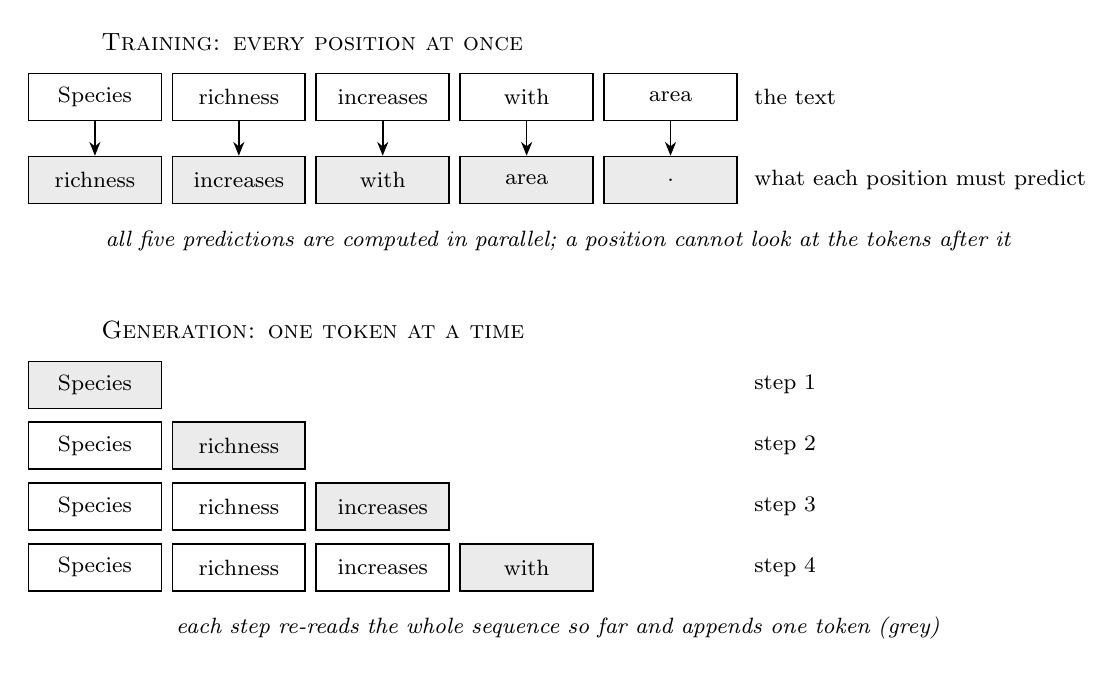
\begin{tikzpicture}[tok/.style={box, minimum width=48pt, minimum height=17pt,
                                inner sep=2pt, font=\footnotesize},
                    grey/.style={fill=lightgrey}]
  % Training
  \node[title, anchor=west] at (0,0) {Training: every position at once};
  \foreach \w [count=\i] in {Species, richness, increases, with, area}
    \node[tok] (a\i) at ({(\i-1)*52pt}, -20pt) {\w};
  \foreach \w [count=\i] in {richness, increases, with, area, .}
    \node[tok, grey] (p\i) at ({(\i-1)*52pt}, -50pt) {\w};
  \foreach \i in {1,...,5} \draw[->] (a\i) -- (p\i);
  \node[tag, anchor=west] at (236pt,-20pt) {the text};
  \node[tag, anchor=west] at (236pt,-50pt) {what each position must predict};
  \node[note, anchor=west, text width=330pt] at (0,-72pt)
    {all five predictions are computed in parallel; a position cannot look at the tokens after it};
  % Generation
  \node[title, anchor=west] at (0,-104pt) {Generation: one token at a time};
  \node[tok, grey] at (0,-124pt) {Species};
  \node[tok] at (0,-146pt) {Species}; \node[tok, grey] at (52pt,-146pt) {richness};
  \node[tok] at (0,-168pt) {Species}; \node[tok] at (52pt,-168pt) {richness};
    \node[tok, grey] at (104pt,-168pt) {increases};
  \node[tok] at (0,-190pt) {Species}; \node[tok] at (52pt,-190pt) {richness};
    \node[tok] at (104pt,-190pt) {increases}; \node[tok, grey] at (156pt,-190pt) {with};
  \foreach \k/\y in {1/-124,2/-146,3/-168,4/-190}
    \node[tag, anchor=west] at (236pt,\y pt) {step \k};
  \node[note, anchor=west, text width=330pt] at (0,-212pt)
    {each step re-reads the whole sequence so far and appends one token (grey)};
\end{tikzpicture}
\end{document}
